\documentclass[thesis.tex]{subfiles}
\begin{document}
The (theoretical) results from the previous chapter show the potency of the equilibrated residual estimator.
Most results are upper- or lower bounds and some of these still depend on unknown constants.
To address these uncertainties we would like to measure the performance in practice.
In particular, how tight is the error bound given by the equilibrated residual estimator?
What is the practical convergence rate of AFEM driven by the equilibrated estimator?
How do the equilibrated and classical estimator --- both optimal AFEM drivers --- compare to eachother?

We will start this chapter by discussing some implementationional issues, after which we will gather numerical results to
answer the proposed questions. MATLAB \cite{MATLAB:2015} will be used for the actual implementation. We also
make extensive use of iFEM \cite{chenifem}, a general framework for adaptive finite element methods. 

\section{Ern and Volharik's construction}
\textcolor{blue}{Misschien moet deze sectie in het vorige hoofdstuk?}
The equilibration method is based on constructing the difference flux $\vsig^\triangle 
= \nabla U_h - \v{\sigma}$, 
with $\vsig^\triangle$ from the broken Raviart-Thomas space $\RT_p^{-1}(\T_h)$. 
An equivalent equilibration construction is given by Ern and Volharik in \cite{ernequil}. They
propose constructing the actual flux $\vsig \in \RT_p(\T_h)$ instead of the difference, with
a method that allows for a direct implementation.

Define $\v{\zeta_a} := \v{\sigma_a} - \psi_a \nabla U_h$ in notation of \cite{ernequil}. By the partition of unity we have 
$\sum_{a \in \V} \v{\zeta_a} = \vsig^\triangle - \nabla U_h$. Rewriting the characteristic property \eqref{eq:sigmadefdisc} of flux $\v{\sigma_a}$ yields
\begin{align*}
  -\ip{\v{\sigma_a}, \nabla v}_{\w_a}  = \ip{\tilde r_a, v} &=  \ip{Q_a(\psi_a f), v}_{\w_a} - \ip{\nabla U_h, \nabla \left(\psi_a v\right)}_{\w_a} \\
  &=  \ip{Q_a(\psi_a f) - \nabla \psi_a \cdot \nabla U_h, v}_{\w_a} - \ip{\psi_a \nabla U_h, \nabla v}_{\w_a} \quad \forall v \in H_\star^1(\w_a).
\end{align*}
This holds if and only if  we have for all $v \in H_\star^1(\w_a)$ that
\begin{equation}
  \label{eq:defzeta}
  \ip{Q_a(\psi_a f) - \nabla \psi_a \cdot \nabla U_h, v}_{\w_a} = - \ip{\v{\sigma_a} - \psi_a \nabla U_h, \nabla v}_{\w_a} = - \ip{\v{\zeta_a}, \nabla v}_{\w_a}.
\end{equation}
Notice\footnote{
For $a\in \V_h^{bdr}$ it is clear that $C_c^{\infty}(\w_a) \subset H_\star^1(\w_a)$. For $a \in \V_h^{int}$, take $v \in C_c^{\infty}(\w_a)$ and consider $v - v_{\w_a} \in H_\star^1(\w_a)$. Plugging $v - v_{\w_a}$ into the equation \eqref{eq:defzeta} and using orthogonality relations shows that actually $ - \ip{\v{\zeta_a}, \nabla v} = \ip{Q_a(\psi_a f) - \nabla \psi_a \cdot \nabla U_h, v}_{\w_a}$ for $v \in C_c^{\infty}(\w_a)$.}
that the weak divergence apparently satisfies  $\div \v{\zeta_a} = Q_a(\psi_a f) - \nabla \psi_a\cdot \nabla U_h$.
The latter is a $L^2(\w_a)$ function, and since
%\footnote{We know that $\v{\sigma_a}\in \RT_{p,0}^{-1}(\w_a)$. Moreover $\nabla U_h \in \RT_p^{-1}(\w_a)$ and since $\psi_a$ vanishes on $\partial \w_a \setminus \partial \O$ we can conclude that $\psi_a\nabla U_h \in \RT_{p,0}^{-1}(\w_a)$.
 $\v{\sigma_a},\psi_a\nabla U_h \in \RT_{p,0}^{-1}(\w_a)$ we conclude
\[
  \v{\zeta_a} \in H(\div; \w_a) \cap \RT_{p,0}^{-1}(\w_a) = \RT_{p,0}(\w_a).
\]

Constructing $\v{\sigma_a} - \psi_a\nabla U_h$ is therefore equivalent to finding $\v{\zeta_a} \in \RT_p(\w_a)$ with
$\div \v{\zeta_a} = Q_a(\psi_af) - \nabla \psi_a \cdot \nabla U_h$ and minimal $\uanorm{\v{\zeta_a} + \psi_a \nabla U_h}_{\w_a}$.
This latter problem can be turned into a system of equations. 
\begin{thm}
  For vertex $a \in \V_h$ the function $\v{\zeta_a} \in \RT_{p,0}(\w_a)$ can be found by solving
  \begin{subequations}
    \label{eq:systemzeta}
  \begin{alignat}{3}
    \ip{\v{\zeta_a}, \v{\tau}}_{\w_a} - \ip{\div \v{\tau}, {\lambda_a}}_{\w_a} &= - \ip{\psi_a \nabla U_h, \v{\tau}}_{\w_a} && \quad \forall \v{\tau} \in \RT_{p,0}(\w_a),\label{eq:systemzeta1}\\
    \ip{\div \v{\zeta_a}, q_a}_{\w_a} &= \ip{\psi_a f - \nabla \psi_a \cdot \nabla U_h, q_a}_{\w_a} && \quad \forall q_a \in \QQ(\w_a), \label{eq:systemzeta2}
  \end{alignat}
\end{subequations}
  for the pair $(\v{\zeta_a}, {\lambda_a}) \in \RT_{p,0}(\w_a) \times \QQ(\w_a)$.
  With $\QQ(\w_a)$ a polynomial subspace given by
  \[
    \QQ(\w_a) := \left[\begin{aligned}
        &\set{q \in \P_p^{-1}(\w_a) : q_{\w_a} = 0}  &\quad a \in \V_h^{int},\\
        &\set{q \in\P_p^{-1}(\w_a)}&\quad a \in \V_h^{bdr}.
      \end{aligned}
      \right.
  \]
\end{thm}
\begin{proof}
  We will start by showing that the characteristic property \eqref{eq:defzeta}  of $\v{\zeta_a}$ is equivalent to \eqref{eq:systemzeta2}.
  Here we will use that $Q_a$ is the $L_2$-orthogonal projector on the broken polynomial space $\P_p^{-1}(\w_a)$.  Fix $v \in H_\star^1(\w_a)$, 
  since $\v{\zeta_a} \in \RT_{p,0}(\w_a)$ we know that $\div \v{\zeta_a} \in \P_p^{-1}(\w_a)$, and thus that $Q_a( \div \v{\zeta_a} )= \div \v{\zeta_a}$. Combined with orthogonality of the projector the right hand side of \eqref{eq:defzeta} reads
  \[
    -\ip{\vzeta, \nabla v}_{\w_a} = \ip{\div \v{\zeta_a}, v}_{\w_a} = \ip{ Q_a(\div \v{\zeta_a}), v}_{\w_a} = \ip{\div \v{\zeta_a}, Q_a(v)}_{\w_a}.
  \]

  Something similar for the left hand side of \eqref{eq:defzeta} holds. The expression $\nabla \psi_a \cdot \nabla U_h$ is part of
  $\P_p^{-1}(\w_a)$, since $\psi_a \in \P_1(\w_a)$ and $U_h \in \P_{p}(\w_a)$. Similar steps as before give, 
  \begin{align*}
    \ip{Q_a(\psi_a f) - \nabla \psi_a \cdot \nabla U_h, v}_{\w_a} &= \ip{Q_a(\psi_a f) - Q_a\left(\nabla \psi_a \cdot \nabla U_h\right),v}_{\w_a}\\
    &= \ip{Q_a\left(\psi_a f - \nabla \psi_a \cdot \nabla U_h\right), v}_{\w_a}\\
    &= \ip{\psi_a f - \nabla \psi_a \cdot \nabla U_h, Q_a(v)}_{\w_a}.
  \end{align*}
  From this we conclude that \eqref{eq:defzeta} is equivalent to
  \[
    \ip{\div \v{\zeta_a}, q_a}_{\w_a} = \ip{\psi_a f - \nabla \psi_a \cdot \nabla U_h, q_a} \quad \forall q \in Q_a\left(H_\star^1(\w_a)\right).
  \]
  The equivalence is completed by  noting that $Q_a\left(H_\star^1(\w_a)\right) = \QQ(\w_a)$ for both interior and boundary vertices $a$.

  \textcolor{blue}{
  For $a \in \V_h^{int}$ this is obvious, 
  since $\ip{Q_a(v), 1}_{\w_a} = \ip{v,Q_a(1)}_{\w_a} = v_{\w_a} = 0$ for $v \in H_\star^1(\w_a)$.
  On the other hand, for $a \in \V_h^{bdr}$ pick $q_a \in \P_p^{-1}(\w_a)$.
  Can we find a sequence $v_\epsilon \in H_\star^1(\w_a)$ such that $\norm{Q_a(v_\epsilon) - q_a}_{\w_a} \to 0$ 
  and $v_\epsilon \to v \in H_\star^1(\w_a)$. If so, we have $Q_a(v) = q_a$ for a $v \in H_\star^1(\w_a)$ and thus we may conclude
  that $Q_a\left(H_\star^1(\w_a)\right) = \QQ(\w_a)$. Probably possible using some mollifier.  }

  Next we tackle rewriting the minimizing problem. By the polarization identity
  \[
    \uanorm{\v{\zeta_a} + \psi_a \nabla U_h}_{\w_a}^2 = \uanorm{\v{\zeta_a}}_{\w_a}^2 + \norm{\psi_a \nabla U_h}^2_{\w_a} + 2 \ip{\v{\zeta_a}, \psi_a \nabla 
    U_h}_{\w_a}.
  \]
  Now $\psi_a \nabla U_h$ is fixed,  so minimizing $\uanorm{\v{\zeta_a} + \psi_a \nabla U_h}_{\w_a}$ for $\vzeta$ is equivalent to minimizing
  \[
    \frac{1}{2} \uanorm{\v{\zeta_a}}^2_{\w_a} + \ip{\v{\zeta_a}, \psi_a \nabla U_h}_{\w_a}.
  \]

There exists a basis $\set{\v{\tau_1},\dots, \v{\tau_n}}$ of $\RT_{p,0}(\w_a)$ and
  a basis $\set{q_1, \dots, q_M}$ of $\QQ(\w_a)$. Express the solution $\v{\zeta_a}$ in this basis  and use the previous paragraphs
  to  see that solving $\v{\zeta_a} \in \RT_{p,0}(\w_a)$ is
  equivalent to finding coefficients $\v{c} \in \R^n$ that minimize 
  \[
    J(\v{c}) := \frac{1}{2} \norm{\sum c_i \v{\tau_i}}^2_{\w_a} + \ip{\sum c_i \v{\tau_i}, \psi_a \nabla U_h}_{\w_a}
  \]
  subject to the constraint $G(\v{c}) = \v{0}$, where
  \[
    G_k(\v{c}) = \ip{\div \sum c_i \v{\tau_i}, q_k}_{\w_a} - \ip{\psi_a f - \nabla \psi_a \cdot \nabla U_h, q_k}_{\w_a}  \quad k \in \set{1, \dots, M}.
  \]
  This appears like a classical optimisation problem, and we can solve it using the Lagrange multiplier. 
  Let $\v{c}$ be a local minimum of $J$ satisfying the optimization constraint, then
  exists a Lagrange multiplier $\v{\lambda} \in \R^{M}$ such that 
   \begin{equation}
     \label{eq:lagrange}
     \nabla J(\v{c}) + \sum \lambda_k \nabla G_k(\v{c}) = 0\quad \text{and} \quad G(\v{c}) = 0.
   \end{equation}
   Calculating the partial derivatives of $J$ and $G_k$ for $c_j$ with $j=1,\dots, n$ gives
   \begin{align*}
     \frac{\partial J}{\partial c_j} &= \ip{ \sum c_i \v{\tau_i}, \v{\tau_j}}_{\w_a} + \ip{\v{\tau_j}, \psi_a \nabla U_h}_{\w_a},\\
     \frac{\partial G_k}{\partial c_j} &= \ip{\div \v{\tau_j}, q_k}_{\w_a}.
   \end{align*}
   Plug these derivatives into the Lagrange equation \eqref{eq:lagrange}; one directly sees that
   solving $(\v{c}, \v{\lambda})$ from \eqref{eq:lagrange} is equivalent to solving $(\v{\zeta_a}, \v{\lambda_a})$ from
   the system \eqref{eq:systemzeta} by setting $(\v{\zeta_a},{\v{\lambda_a}}) = (\sum c_i \tau_i, \sum \lambda_k q_k)$.
   In other words, every $\v{\zeta_a}$ that attains a local minimum indeed solves the sytem.

  The approach above does not provide us with uniqueness of $\v{\zeta_a}$. For this we require more evolved optimisation theory. 
  Finding the pair $(\v{\zeta_a}, {{\lambda_a}}) \in \RT_{p,0}(\w_a) \times \QQ(\w_a)$ that solves the system 
  \eqref{eq:systemzeta} is actually a \emph{saddle point problem} (cf. \cite{brezzimixed, braess2007finite}).
  That is, it fits in the general framework of finding $(u, \lambda) \in X \times M$ for Hilbert spaces $X$ and~$M$~with
    \begin{align*}
      a(u,v) + b(v,\lambda) &= \ip{f,v} \quad \forall v \in X,\\
      b(u, \mu) &= \ip{g,\mu} \quad \forall \mu \in M,
    \end{align*}
    for $f \in X', g \in M'$ and continuous bilinear forms $a: X \times X \to \R, b : X \times M \to \R$.
    The main result about saddle point problems \cite[Thm~4.3]{braess2007finite} provides sufficient conditions under which there 
    is a unique solution $(u, \lambda)$ to the saddle point problem such that~$u$ is also the unique minimizer of 
    $\frac{1}{2} a(u,u) - \ip{f,u}$. First, the bilinear form $a(\cdot, \cdot)$ should be symmetric and coercive on
    the set of functions $V := \{v \in X : b(v, \cdot) = 0\}$.
    Secondly, the bilinear form $b(\cdot, \cdot)$ must satisfy the inf-sup condition: 
    \[
      \exists \beta > 0, \inf_{\mu \in M} \sup_{v \in X}\frac{b(v,\mu)}{\norm{v}_X \norm{\mu}_M} \geq \beta.
    \]

    Fit the general framework on our system \eqref{eq:systemzeta}; we 
    have $a(\v{\zeta_a},\v{\tau}) = \ip{\v{\zeta_a},\v{\tau}}_{\w_a}$ and $b(\v{\zeta_a},q_a) = \ip{\div \v{\zeta_a},q_a}_{\w_a}$ for $\v{\zeta_a}, \v{\tau} \in \RT_{p,0}(\w_a), q_a \in \QQ(\w_a)$. For $\v{\tau} \in V$ we have by definition $\ip{\div \v{\tau}, q_a}_{\w_a} = 0$ for all $q_a \in \QQ(\w_a)$, which implies that $\div \v{\tau} = 0$ since $\div \v{\tau} \in \QQ(\w_a)$. Coercivity of  $a(\cdot, \cdot)$ on $V$ therefore follows easily,
    \[
      a(\v{\tau},\v{\tau}) = \ip{\v{\tau},\v{\tau}}_{\w_a} = \norm{\v{\tau}}^2_{\w_a} = \norm{\v{\tau}}^2_{\w_a} + \norm{\div \v{\tau}}^2_{\w_a} = \norm{\v{\tau}}^2_{H(\div; \w_a)}.
    \]
    For the inf-sup condition we consider the following operator,
    \[
      B : \RT_{p,0} \to \QQ(\w_a)' : \, \, \tau \mapsto \ip{\div \tau, \cdot}_{\w_a}.
    \]
    Given $q_a \in \QQ(\w_a)$ there exists $ \v{\tau_a} \in \RT_{p,0}(\w_a)$  such that 
    $\div  \v{\tau_a} = q_a$ (cf. proof of Theorem~\ref{thm:sigmasolvable}).
    By duality this turns $B$ into a surjective map,
    which is equivalent to the inf-sup condition being satisfied (cf. \cite[Thm~4.2.1]{brezzimixed}).
    All in all, we satisfy the necessary conditions and hence we may conclude that there is a unique pair 
    $(\v{\zeta_a}, \lambda) \in \RT_{p,0}(\w_a) \times \QQ(\w_a)$ 
    that solves the system \eqref{eq:systemzeta}, with $\v{\zeta_a}$ the
    unique minimizer of $\uanorm{\v{\zeta_a }+ \psi_a \nabla U_h}_{\w_a}$ subject to $\div \v{\zeta_a} = Q_a(\psi_a f) - \nabla \psi_a \cdot \nabla U_h$.
\end{proof}
{\color{blue}
Why do Ern and Volharik need galerkin orthogonality $\ip{\nabla U_h, \nabla \psi_a}_{\w_a} = \ip{f, \psi_a}_{\w_a}$?
I think they use it to show that the solution of the above system satisfies $(\div \sigma, 1)_K = (f,1)_K$,
which can then be used to show a generalized version of Prager and Synge.

Anyhow, the result in Ern and Volharik is stronger. They just solve the above system for any $p$, regardless of the solution, and
then this solution still satisfies the Synge and Prage upper bound.
}

Since both function spaces in the system \eqref{eq:systemzeta} are finite dimensional, the
system can be reduced to a set of equations over the bases of $\RT_{p,0}(\w_a)$ and $\QQ(\w_a)$. Solving this
for each $a \in \V$ provides us with the corresponding $\vzeta$. Using the correspondence with $\vsiga$ we 
directly have the following upper bounds (cf. Theorems~\ref{thm:discsynge} and \ref{thm:discbounds}).
\begin{cor}
  \label{eq:zetaupper}
  Let $\vzeta$ be found by solving \eqref{eq:systemzeta}, then for $\v{\zeta} = \sum_{a \in \V_h} \vzeta$ we have
  \begin{align*}
    \enorm{u - U_h}_{\O}^2 &\leq \sum_{K \in \T_h} \left[ \uanorm{\vzet + \nabla U_h}_{K} + \frac{h_K}{\pi} \uanorm{ (I-Q_a)(\psi_a f)}_{K}\right]^2,\\
    \enorm{u - U_h}_{\O}^2 &\leq 3 \sum_{a\in \V_h}\left[\norm{\vzeta + \psi_a \nabla U_h}_{\w_a} + C_{FP,\w_a} h_{\w_a} \norm{(I - Q_a)(\psi_a f)}_{\w_a}\right]^2.
  \end{align*}
\end{cor}


%\section{Bases for $\RT_{p,0}(\w_a)$ and $\QQ(\w_a)$}
\section{Raviart-Thomas space}
The findings in the previous section provide us with the necessary steps for implementation of the
estimator. In particular we must find bases for $\RT_{p,0}(\w_a)$ and $\QQ(\w_a)$. We will give a short
intermezzo deriving some theory for this first space. 

Consider an arbitrary domain $ \O \subset \R^2$ with triangulation $ \T$, vertices $ \V$, et cetera.
We will start by examining the Raviart-Thomas space $\RT_p( \T)$, without the boundary conditions,
generated by the Raviart-Thomas element.
Recall that elements are formally represented by a triplet $(K, \mathcal{P}, \mathcal{N})$ (cf. \S\ref{sec:deffem}). For
the construction of the Raviart-Thomas space ~$\RT_p( \T)$
we obviously have $\mathcal{P} := \RT_p(K)$.
We are left with the task of finding suitable nodal variables $\mathcal{N}$ that ensure $H(\div;  \O)$ conformity of the entire space.
For this latter constraint we will use the following characterization of $H(\div;  \O)$.
\begin{thm}
  \label{thm:rtjump}
  The Raviart-Thomas space $\RT_p( \T)$  can be characterized by
  \[
    \RT_p( \T) := H(\div;  \O) \cap \RT_p^{-1}( \T)  = \set{\vsig \in \RT_p^{-1}( \T) : \llbracket \vsig \rrbracket = 0 \, \text{ in } L^2(e) \quad \forall e \in \E^{int}}.
  \]
\end{thm}
\begin{proof}
  We show the inclusion "$\supset$". That is, let $\vsig \in \RT_p^{-1}( \T)$ be given such that $\llbracket \vsig \rrbracket$
  vanishes on all interior edges. We have to show that $\vsig$ has a weak divergence in $L^2( \O)$.
  Let $\f \in D( \O)$ be given, then
  \begin{align*}
    - \int_{ \O}  \nabla \f \cdot \vsig &= - \sum_{K \in  \T} \int_K \nabla \f \cdot \vsig \\
    &=  \sum_{K \in  \T} \int_K \f \cdot \nabla \vsig - \int_{\partial K} \f \vsig \cdot n\\
    &=  \int_{ \O} \f \cdot \nabla \vsig - \sum_{e \in  \E^{int}} \int_e \f \llbracket \vsig \rrbracket = \int_{ \O} \f \cdot \nabla \vsig.
  \end{align*}
  Where we used that $\f$ vanishes on the boundary, whilst $\llbracket \vsig \rrbracket$ vanishes on interior edges.
  The result follows since $\nabla \vsig \in L^2( \O)$, hence we may conclude that $\vsig \in H(\div;  \O)$.

  The other inclusion follows similarly (cf. \cite[Thm~3.2]{gaticasimple}).
\end{proof}

For elements $K \in  \T$ we have $\RT_p(K) := \left[ \P_p(K)\right]^2 + \P_p(K)\v{x}$.
Write $\wt \P_p(K)$ for polynomials of exactly degree $p$, then one easily proves the decomposition
$\RT_p(K) = \left [\P_p(K)\right]^2 \oplus \wt \P_p(K) \v{x}$.
From this it follows that 
\[
  \dim{\RT_p(K)} = 2 \dim{\P_p(K)}+ \dim{\wt \P_p(K)} = 2 {2 + p \choose p} + {2 + p - 1 \choose p} = (p+1)(p+3).
\]
Moreover we have the following (unisolvent) characterisation.
\begin{thm}
  Let $K \in  \T$ and $\vsig \in \RT_p(K)$ be given such that
  \begin{alignat*}{2}
    \ip{\vsig \cdot n_e, q}_e &= 0 \quad \forall q \in \P_p(e), &&\quad \forall \text{edge } e \subset \partial K,\\
    \ip{\vsig, \vtau}_K &= 0 \quad \forall \vtau \in \left[\P_{p-1}(K)\right]^2, &&\quad p \geq 1.
  \end{alignat*}
  Then $\vsig \equiv 0$ in $K$.
\end{thm}
\begin{proof}
  Counting the dimensions shows that the number of equations equals the dimension of $\RT_p(K)$. Moreover, one easily sees that $\vsig \cdot n_e \in \P_p(e)$, so that by first equation $\vsig \cdot n_e$ vanishes on all edges of $K$.

  Let $p \geq 1$, then for $q \in \P_p(K)$ we have $\nabla q \in \left[\P_{p-1}(K)\right]^2$, and by the divergence theorem this gives that
  $\ip{\div \vsig, q}_K = - \ip{\vsig, \nabla q}_K + \ip{\vsig \cdot n, q}_{\partial K} = 0$. Since $\div \vsig \in P_p(K)$, we
  may conclude that $\div \vsig = 0$.  Write $\vsig = \v{q} + q_0\v{x}$ for $\v{q} = [q_1, q_2]^\top$ with $q_1, q_2  \in\P_p(K)$ and $q_0 \in  \wt \P_p(K)$. Using that $\div \vsig =0$ gives us
  \[
    0 = \div \vsig = \div \v{q} + \div \left(q_0 \v{x}\right) = \div \v{q} + (2 + p) q_0 \implies (2 + p) q_0 = - \div \v{q} \in \P_{p-1}(K).
  \]
  Since $q_0 \in \wt \P_p(K)$ this shows that $q_0 \equiv 0$, and thus that $\vsig = \v{q}$.

  For every edge $e \in \partial K$ we have $\v{q} \cdot n_e =0$ on $e$ for a polynomial $\v{q} \cdot n_e \in \P_p(K)$. Every
  polynomial $p \in \P_{p-1}(K)$ satisfies
  \[
    \ip{\v{q} \cdot n_e, p}_K = \ip{\v{q}, \v{p} \cdot n_e}_K = 0, \quad \v{p} = [p,p]^\top \in \P_{p-1}(K).
  \]
  Since $\v{q}\cdot n_e$ vanishes on $e$ we decompose $\v{q}\cdot n_e = Lp$ for a polynomial $p \in \P_{p-1}$ and $L$ the hyperplane of $e$ \cite[Lem~3.1.10]{brenner}. Using this polynomial $p$ in the above identity then shows
  \[
    0 = \ip{\v{q}\cdot n_e, p}_K = \ip{Lp, p}_K = \ip{L,p^2}_K.
  \]
  On the other hand we have $L > 0$ or $L < 0$ on $K$. Therefore we must conclude that $p = 0$, and thus that $\v{q}\cdot n_e$ vanishes
  on the entire element $K$. Since this holds for all edge normals $n_e$ we conclude that $\v{q} = 0$ on $K$.
\end{proof}
The number of equations in the previous theorem is exactly equal to $\dim{\RT_p(K)}$, and therefore provides us with a
set of nodal variables. That is, for each edge $e$ let $\set{q_{e,1},\dots, q_{e,m}}$ be a basis of $\P_p(e)$, and pick
 $\set{\vtau_1, \dots, \vtau_r}$ as a  basis for $\left[\P_{p-1}(K)\right]^2$. 
 Define linear functionals on $\RT_p(K)$ associated to edges and elements by
\begin{equation}
  \label{eq:nodalrt}
  \begin{alignedat}{2}
    N_{e,i}(\vsig) &= \ip{\vsig \cdot n_e, q_{e,i}}_e && \quad 1 \leq i \leq m,  e \subset \partial K\\
    N_{K,j}(\vsig) &= \ip{\vsig, \vtau_j}_K &&\quad 1 \leq j \leq r.
  \end{alignedat}
\end{equation}
The set $\mathcal{N}$ containing all of the above functionals forms a basis for $\RT_p(K)'$, and thus
turns the triplet $(K, \RT_p(K), \mathcal{N})$ into a valid finite element.

\section{Raviart-Thomas basis}
We have formally introduced an Raviart-Thomas element $(K, \RT_p(K), \mathcal{N})$. How can we glue these elements
together to form a basis for the Raviart-Thomas $\RT_p(\T)$? In particular we must ensure $H(\div; \O)$-conformity.

For simplicity we take two adjoint Raviart-Thomas elements $K_1, K_2 \in  \T$ with common edge $e = K_1 \cap K_2$.
From the characterization in Theorem~\ref{thm:rtjump} we know that
\[
\RT_p(K_1 \cup K_2) = \set{\vsig \in \RT_p^{-1}(K_1 \cup K_2) : \llbracket \vsig \rrbracket = 0 \text{ in } L_2(e)}.
\]
Pick $\vsig \in \RT_p^{-1}(K_1 \cup K_2)$ and let $n_e$ be the unit outward normal on $e$ for element $K_1$,
then the conformity condition can be rewritten as
\[
  0 = \llbracket \vsig \rrbracket  = \vsig|_{K_2} \cdot  n_e - \vsig|_{K_1} \cdot n_e.
\]
As $\vsig|_{K_1} \cdot n_{e}, \vsig|_{K_2} \cdot n_{e}$ are both elements in $\P_p(e)$ we see that 
the  above condition is equivalent to requiring
\[
  \ip{\vsig|_{K_2} \cdot n_e, q} = \ip{\vsig|_{K_1} \cdot n_e, q} \quad \forall q \in \P_p(e).
\]
This is satisfied exactly if the edge-related nodal variables of $K_1$ and $K_2$ coincide for $\vsig$.

The above observation is easily extended to the entire Raviart-Thomas space $\RT_p( \T)$.
That is, the space consists of those functions from $\RT_p^{-1}( \T)$ for which all the edge-related
nodal variables of two adjoint elements coincide. For each element $K \in  \T$, denote $\phi^K_{e,i}$ and $\phi^K_{K,j}$
for the nodal basis with respect to \eqref{eq:nodalrt}. A basis for the entire space is then found by
glueing together edge related functions. To be precise, a basis for $\RT_p( \T)$ is given by
\begin{equation}
  \label{eq:basisrt}
  \{\phi^K_{K, j} : K \in  \T, 1 \leq j \leq r\} \cup \{\phi^{K^1}_{e,i} + \phi^{K^2}_{e,i}: K_1, K_2 \in  \T, e = K_1 \cap K_2, 1 \leq i \leq m\},
\end{equation}
with all basis functions naturally extended to $\O$.

Now suppose that we are interested in $\RT_{p,0}( \T) = \set{ \vsig \in \RT_{p,0}( \T) : \vsig \cdot n = 0 \text{ on } \partial  \O}$.
Such a boundary condition is easily incorporated into the basis \eqref{eq:basisrt}; one just has to remove all the basis functions associated
to boundary edges.

\section{Explicit bases lowest order}
With this (general) information on the  Raviart-Thomas space in mind we will reconsider the
system of equations \eqref{eq:systemzeta} defining $\vzeta$. For simplicity we will start
with a lowest order solution of this system, that is $p=0$.  

\subsection{Raviart-Thomas}
For the lowest order Raviart-Thomas space we only have edge related nodal variables.
Let $K$ be a triangle with vertices $\set{v_1, v_2, v_3}$ and the opposite edges given by $\set{e_1, e_2, e_3}$.
A basis for $\P_0(e_i)$ is simply the constant function~$\1$.
Consider the nodal basis function $\v{\phi_1} \in \RT_0(K)$ given by the nodal variable associated with $e_1$.
By construction this is given as a solution of
\[
  \int_{e_1} \v{\phi_1}\cdot n_{e_1} = 1 \quad \text{ and } \int_{e_2} \v{\phi_1} \cdot n_{e_2} = 0 = \int_{e_3} \v{\phi_1} \cdot n_{e_3}.
\]

This can be solved geometrically; as $v_i$ lies opposite of $e_i$, we have $(\v{x} - v_1) \perp n_{e_2}$ for $\v{x} \in e_2$ and similarly $(\v{x} - v_1) \perp  n_{e_3}$ for $\v{x} \in e_3$.
From this we deduce that $\v{\phi_1} = \alpha (\v{x} - v_1)$ for some $\alpha$. Pick a  point $\v{x}$ on the hyperplane given by $e_1$ such that
$(\v{x} - v_1) \perp e_1$, then from vector algebra we see
\[
  1 = \alpha(\v{x} - v_1)\cdot n_{e_1} = \alpha \norm{\v{x} - v_1}\norm{n_{e_1}} \cos \theta = \alpha \norm{\v{x} - v_1}.
\]
This latter norm is also known as the \emph{height} $h_1$ of $e_1$. From well known formula $\frac{1}{2} h_1 \vol(e_1) = \vol(K)$
we observe that $\alpha = \frac{\vol(e_1)}{2\vol(K)}$; a  basis for $\RT_0(K)$ is given by
\[
  \v{\phi_i} = \frac{1}{2}\frac{\vol(e_1)}{\vol(K)}( \v{x} - v_i).
\]

Next we consider the global space $\RT_0(\T)$. For this lowest order Raviart-Thomas space all the degrees of freedom are associated
to edges. For every shared edge $e$ we must fix a \emph{global} orientation of $n_e$. After fixing such an orientation we can (uniquely) identify the adjacent elements by $K_+$ and $K_-$; with $K_+$ the element for which $n_e$
is an outward pointing normal vector. Similarly write $v_+, v_-$ for the vertex opposite of $K_+$ resp $K_-$, then the
basis function associated to $e$ is given by
\[
  \v{\phi_e}(\v{x}) = \begin{cases}
    \frac{1}{2}\frac{\vol(e)}{\vol(K_+)}( \v{x} - v_+) & \v{x} \in K_+\\
    - \frac{1}{2}\frac{\vol(e)}{\vol(K_-)}( \v{x} - v_-) & \v{x} \in K_-.
\end{cases}
\]
The extra boundary constraints needed in \eqref{eq:systemzeta} are easily incorporated; a basis for $\RT_{0,0}(\w_a)$ is simply given
by removing the basis functions associated to edges $\partial \w_a \setminus \partial \O$.
\subsection{Polynomial basis}
\todo{Betere titel?}
The system \eqref{eq:systemzeta} defines the polynomial space $\QQ(\w_a) \subset \P_0^{-1}(\w_a)$. For boundary
vertices we can simply take the constant functions $\1$ on each of the elements. For an interior vertex $a \in \V^{int}$
we have the additional mean zero constraint, i.e.
\[
  \QQ(\w_a) = \set{q \in \P_0^{-1}(\w_a) : \ip{q,1}_{\w_a} = 0}.
\]
Write $K_1,\dots, K_n$ for the elements in the patch $\w_a$. A function $p \in \P_0^{-1}(\w_a)$ is constant
with value $p_i$ on $K_i$. The mean zero condition translates into
\[
  0 = \ip{p,\1}_{\w_a} = \sum_{i =1}^n \ip{p_i, \1}_{K_i} = \sum_{i=1}^n p_i \vol(K_i).
\]
Therefore a basis for $\QQ(\w_a)$ is given by $q_1, \dots, q_{n-1}$ with
\[
  q_i(x) = \begin{cases}
    \vol(K_n) & \quad x \in K_i\\
    -\vol(K_i) & \quad x \in K_n.
  \end{cases}
\]
Unfortunately this is not an orthogonal basis, but for out test purposes it suffices.
\section{Implementation details}
Lets consider an implementation that finds $\vzeta$ by solving the system \eqref{eq:systemzeta}. 
For simplicity of the implementation we let $p=0$, with $f$ piecewise constant and we take $U_h$ to be the \emph{linear} Lagrange finite element solution on for some triangulation $\T$. Since $U_h$ is of polynomial degree $1$ we cannot expect the theory from the previous chapter
to hold. One can still proof the solution $\vzeta$ of \eqref{eq:systemzeta} gives an upper bound for $\enorm{u - U}_\O$, but
the efficiency result is no longer true. 

Implementation of the estimator $\vzeta$ for $p=0$ follows now quite easily. 
Start with an interior vertex $a \in \V$ we must solve $(\vzeta, \lambda_a) \in \RT_{0,0}(\w_a)\times \QQ(\w_a)$ from the system
\begin{equation}
  \label{eq:systemp0}
  \begin{alignedat}{3}
    \ip{\v{\zeta_a}, \v{\tau}}_{\w_a} - \ip{\div \v{\tau}, {\lambda_a}}_{\w_a} &= - \ip{\psi_a \nabla U_h, \v{\tau}}_{\w_a} && \quad \forall \v{\tau} \in \RT_{0,0}(\w_a),\\
    \ip{\div \v{\zeta_a}, q_a}_{\w_a} &= \ip{\psi_a f - \nabla \psi_a \cdot \nabla U_h, q_a}_{\w_a} && \quad \forall q_a \in \QQ(\w_a).
  \end{alignedat}
\end{equation}
  Let $n$ be the number of triangles in $\w_a$.
  For the space $\RT_{0,0}(\w_a)$ we have one degree of freedom associated to every interior edge, and thus $n$ basis functions $\vtau_i$. The space $\QQ(\w_a)$ has $n-1$ basis functions $q_k$.  To solve the above system we must calculate four type of basis interactions:
  \begin{equation}
    \label{eq:basinact}
    \ip{\vtau_i, \vtau_j}_{\w_a}, \, \ip{\div \vtau_i, q_k}_{\w_a}, \, \ip{\psi_a \nabla U_h, \vtau_i}_{\w_a}, \text{ and } \ip{\psi_a f - \nabla \psi_a \cdot \nabla U_h, q_k}_{\w_a}.
  \end{equation}
  The standard finite element approach is to decompose these inner products over the elements $K$, and then use an affine transformation
  to reduce the calculations to interactions on one reference triangle $\hat K$. Unfortunately these transformations do no preserve
  normal components; the result of an affine transformation does not need to lie in $H(\div; \hat K)$. This can be solved 
  by using the Piola transformation instead \cite[\S2.1.3]{brezzimixed}. 
  
  We opt not to follow this approach and instead solve the inner products by quadrature. Since  $f$ is piecewise constant, all of the
  terms in \eqref{eq:basinact} are actually polynomials of degree less or equal 2. 
  The edge-midpoint quadrature rule is exact for polynomials for quadratic polynomials, and hence provides us with an easy
  method to calculate the integrals. Denote the edge-midpoints of a triangle $K$ by $m_i$, then this quadrature is given by
  \[
    \int_K p = \frac{\vol(K)}{3} \sum_{k=1}^3 p(m_k)\quad \forall p \in \P_2(K).
  \]
  Applying this to the first term in \eqref{eq:basinact} gives 
  \[
  \ip{\vtau_i, \vtau_j}_{\w_a} = \sum_{K \subset \w_a} \frac{\vol(K)}{3}\sum_{k=1}^3 \vtau_i(m_k) \cdot \vtau_j(m_k).
  \]
  The other terms decompose similarly.  
  
  Carefully evaluating the explicit formulas in the above quadrature provides us with with the interactions \eqref{eq:basinact}.
  Recall that one had to chose an global orientation for each of the edge normal vectors. For this we make clever
  use of the framework provided by iFEM, see \cite{chenifem} for an in-depth overview of this framework. Collect
  the resulting values from \eqref{eq:basinact} into the matrix analogue of the system \eqref{eq:systemp0}. Solving
  this system then provides us with the basis coefficients of $\vzeta$. Using a local-to-global mapping of edge coefficients
  then allows for iterative construction of $\v{\zeta} = \sum_{a \in \V} \vzeta$. 

  The construction of $\vzeta$ for a boundary vertex $a \in \V^{bdr}$ is similar; the interactions
  are just calculated for a slightly different set of functions. Since $f$ is piecewise constant
  we do not have data data oscillation; and the upper bounds in \eqref{eq:zetaupper} are therefore completely given in terms of $\v{\zeta}$ and 
  $\vzeta$. The last step thus consists in calculating the norms $\norm{\v{\zeta} + \nabla U_h}_K$ or $\norm{\vzeta + \psi_a \nabla U_h}_{\w_a}$.
  Since these terms are linear polynomials, we again use edge-midpoint quadrature to exactly calculate them. 

  \section{Numerical results}
  Finally we are able to present some interesting results.  Using the iFEM framework we can easily calculate a linear discrete solution $U_h$ 
  for a given partition. The package ships with an implementation of the \emph{newest vertex bisection} refinement algorithm.\todo{Do
  we need to introduce this anywhere else?} This refinement method bisects triangles and ensures conformity of the resulting triangulation,
  and in addition ensures that the produced triangulation is shape regular with respect to the initial triangulation.
  We will first asses some (normal) finite element solutions.  After this we will
  consider the performance of AFEM driven by the (first order) equilibrated estimator. The results
  will be compared to the classical residual estimator.

  For meaningful results we ideally compare our error bounds to the \emph{exact} error $\enorm{u - U_h}_\O$. Unfortunately this is
  not possible is most situations. If one knows the exact solution $u$ of an interesting problem, then
  the right hand side $f$ of the associated Poisson problem is almost never constant, rendering our implementation useless. 
  We have two ways to overcome this problem. 
  
  The first is to treat the $f$ as if it was piecewise constant; that is, 
  we approximate $\ip{\psi_a f - \nabla \psi_a \nabla U_h, q_k}_K$ by the edge-midpoint quadrature and ignore this approximation error. Similarly we simply replace $\uanorm{f - \div \v{\zeta}}_K$ \todo{this upper bound is not introducd} by its edge-midpoint quadrature. Provided that $f$ is sufficiently smooth, the effects of these extra errors are of higher order $h$, and thus should wary of for small diameter.
  
  The other approach is using a constant $f$, without knowing the exact solution $u$. We propose to approximate the true error $\enorm{u - U_h}_\O$ by replacing $u$ with another finite element solution $\tilde U_h$  --- quite dazzling if one thinks about it.
  To make this work we let $\tilde U_h$ be a solution on a finer triangulation $\tilde \T_h \geq \T_h$, such that
  every element in $\tilde \T_h$ is at least \emph{one} bisections away from its corresponding element in $\T_h$. We have
  \[
    \enorm{u - U_h}_\O \leq \uaenorm{u - \tilde U_h}_{\O} + \uaenorm{U_h - \tilde U_h}_{\O},
  \]
  where we hope --- which is most likely the case if $u$ possesses some smoothness --- that $\uanorm{u - \tilde U_h}_{\O} \ll \uanorm{U_h - \tilde U_h}_{\O}$. The straightforward implementation follows from noting that $U_h$ is also in the finite element spaces of refine triangulations.  iFEM  conviently provides a function that calculates the coefficients of $U_h$ with respect to the linear basis on a refined triangulation.
  \todo{impl iFEM}
  \subsection{Unit square}
  Take $\O = (0,1)\times(0,1)$ with exact solution $u(x,y) = \sin(2\pi x)\sin(2\pi y)$, and thus
  \begin{equation}
    \label{eq:squaresin}
    \begin{alignedat}{2}
      -\Delta u &= 8\pi^2\sin(2\pi x)\sin(2\pi y)  \quad &&\text {in } \Omega, \\
      u &= 0 \quad &&\text{on } \partial\O.
    \end{alignedat}
  \end{equation}
  The exact solution has two peaks and is very smooth. We let iFEM calculate the discrete solutions $(U_k)_{k \geq 0}$ for 
  a sequence of uniformly bisected triangulations, i.e. every triangle is bisected into four subtriangles. It uses third order quadrature to approximate the integrals containing $f$. The produced result is illustrated in Figure~\ref{fig:squareuh}.

  \begin{figure}
    \centering
        \includegraphics[width=.32\linewidth]{mesh_square_1.png}
        \includegraphics[width=.32\linewidth]{mesh_square_3.png}
        \includegraphics[width=.32\linewidth]{square_result_8.png}
        \caption{The finite element solutions $U_k$ for \eqref{eq:squaresin} with  uniformly bisected triangulations, from left to right we have diameters $h = 2^{-1}, 2^{-3}, 2^{-8}$.}
    \label{fig:squareuh}
\end{figure}
The images clearly indicate convergence of the FEM solution. 
As $u \in H^2(\O)$ we expect that $\enorm{u - U_k}_{\O} \lesssim h \abs{u}_{H^1(\O)}$. For uniform refinements this
latter is equivalent to $\enorm{u - U_k}_{\O} \lesssim N^{1/2} \abs{u}_{H^1(\O)}$, with $N$ the total number of vertices.

The iFEM package provides a method to calculate $\enorm{u - U_h}_{\O}$ given the exact $u$, 
and also provides an implementation of the standard residual estimator $\hat \eta_\T(U_h, \T)$.
We compare these against the equilibrated upper bound from \eqref{eq:zetaupper},  i.e.
\[
  \enorm{u - U_h}_{\O} \leq \sqrt{\sum_{K \in \T_h} \left[ \uanorm{\vzet + \nabla U_h}_{K} + \frac{h_K}{\pi} \uanorm{ f - \div\v{\zeta}}_{K}\right]^2}.
\]
We also calculate their efficiency indices as $\enorm{u - U_k} / \eta$. In the equilibrated case we would like this value to be close to one, as this shows tightness of the estimator. In the residual case we have an extra constant in the reliability bound, and thus tightness depends also depends on this (unknown) constant.
The results are given in Figure~\ref{fig:squareerror}. The experimental convergence rate is in line with the theoretical convergence rate.
\begin{figure}
  \centering
  \includegraphics[width=.49\linewidth]{square_norm_slope_7.png}
  \includegraphics[width=.49\linewidth]{square_efficiency_7.png}
  \caption{The left compares the exact error in the energy norm with the standard residual estimator, and the equilibrated residual estimator.
    These are calculated for discrete solutions $U_k$ of \eqref{eq:squaresin} for a sequence of uniformly refined triangulations. 
    The triangle has a slope of $-1/2$.  
  The right figure plots $\enorm{u - U_k} / \eta$; an estimation of the efficiency index.}
  \label{fig:squareerror}
\end{figure}

Even though we calculated the equilibrated estimator for $p=0$, it still proves to be real close to the actual error. The efficiency index
seems to rise, which could be explained by a reduction  in the influence of quadrature errors for smaller diameters. We have the exact solution
$u$ for this system, and thus we can empirically verify the claim that $\enorm{u - U_k}_{\O}$ is more or less equal to $\enorm{U_{k+i} - U_k}_{\O}$ for $i\geq 1$. The results for this problem with $i=1,2,3$ are given in Figure~\ref{fig:squareapprox}. The quality
of the error approximation increases with $i$ as expected. 
\begin{figure}
  \centering
  \includegraphics[width=.49\linewidth]{square_approx_H1_11.png}
  \includegraphics[width=.49\linewidth]{square_approx_H1_rel_11.png}
  \caption{ The exact error $\enorm{u - U_k}_{\O}$ is compared to the approximation $\enorm{U_{k+i} - U_k}_{\O}$ for $i=1,2,3$. The
    left image all of these terms are separately visualised, which results in a cluttered image as expected. The right image
  displays the relative terms, i.e. $\enorm{U_{k+i} - U_k}_{\O} / \enorm{u - U_k}_{\O}$.}
  \label{fig:squareapprox}
\end{figure}


Another Poisson problem for the unit square domain is given by $u(x,y) = 2^{40}x^{10}(1-x)^{10}y^{10}(1-y)^{10}$.
The corresponding right hand side $f$ is a high order polynomial; we let Matlab derivate  it using symbolic calculations. The
solution $u$ has a peak of value $1$ centered around $(\frac{1}{2}, \frac{1}{2})$ and is again very smooth. In Figure~\ref{fig:squareana}
the efficiency indices are given, alongside the relative errors generated by $\enorm{U_{k+i} - U_k}_{\O}$ for this new problem. The 
initial triangulation $\T_0$ is equal the one used in the previous problem.
The efficiency of the equilibrated estimator is less for this problem, which is most likely due to the large oscillation factor,
but it still outperforms the classical residual estimator. 

The behaviour of $\enorm{U_{k+i} - U_k}_\O$ is very similar to that of the previous problem, it appears to be a good estimation of $\enorm{u - U_k}_{\O}$. We will therefore use this in the following problems, due to the absence of an exact solution. 
For practical purposes --- the linear systems rapidly grow in size --- we pick $i=3$, which should be enough for a `true error' indication.
We will write $\wt U_k$ for the discrete solution found on the twice uniformly refined triangulation of $\T_k$.

\begin{figure}
  \centering
  \includegraphics[width=.49\linewidth]{squareana_efficiency_8.png}
  \includegraphics[width=.49\linewidth]{squareana_approx_H1_rel_11.png}
  \caption{Left image compares the efficiency indices of the standard residual estimator with the equilibrated estimator. Right image
  shows the exact error approximation quality.}
  \label{fig:squareana}
\end{figure}

\subsection{Re-entrant corner}
Here $\O = (-1,1)^2\setminus[-1,0]^2$ with right hand side $f = \1$; this is also known as the L-shaped domain. 
The solution $u$ of this problem has a singularity at the origin so
that $u \not \in H^2(\O)$. The theoretical
convergence on uniform refined triangulations is of order $h^{2/3}$. We calculate  discrete solutions $U_k$ for uniform refinements, and use $\uaenorm{\wt U_k - U_k}_\O$ to approximate the true error. 

The results are given in Figure~\ref{fig:lshapeone}. The experimental
convergence of the fem solution appears to match the theoretical convergence. 
The equilibrated residual once again has a better efficiency index than the residual estimator.
There is a drop in terms of efficiency compared to the previous problems. Interestingly, the efficiency of the equilibrated
estimator seems to decrease, whereas the efficiency of the standard estimator is somewhat increasing. 
This might be related to the approximation quality of $\enorm{\tilde U_k - U_k}_{\O}$.

\begin{figure}
  \includegraphics[width=.49\linewidth]{lshapeone_norm_8.png}
  \includegraphics[width=.49\linewidth]{lshapeone_efficiency_8.png}
  \caption{Error estimators and their efficiency for the re-entrant corner problem. The triangle has a slope of $-1/3$.}
  \label{fig:lshapeone}
\end{figure}

\subsection{Crack domain}
A problem with a line singularity is given by the crack domain: take $f = \1$ and
\[
  \O=\{(x,y) \in \R^2 : |x|+|y|<1\}\setminus ([0,1] \times \set{0}).
\]
The exact solution $u$ can be given in polar coordinates, $u(r, \phi) = r^{1/2}\sin(\phi/2) - 1/2 r^2 \sin^2 (\phi)$.
The theoretical convergence rate of uniformly refined triangulations is of order $h^{1/2}$, due to its line singularity. This
domain is implemented by adding the vertex $(1,0)$ twice.  

The results are given in Figure~\ref{fig:crackone}.
There is a drop in the efficiency index compared to the re-entrant corner; this could
be explained by the fact that $u$ is less regular. Again the efficiency of the equilibrated estimator decreases, while the efficiency
of the residual estimator increases.
\begin{figure}
  \includegraphics[width=.49\linewidth]{crackone_norm_8.png}
  \includegraphics[width=.49\linewidth]{crackone_efficiency_8.png}
  \caption{Error estimators and their efficiency for the crack domain problem. The triangle has a slope of $-1/4$.}
  \label{fig:crackone}
\end{figure}

\subsection{Adaptive finite element method}
Due to singularities the convergence rate in these last two examples is not optimal. 
These rates can be increased using the adaptive finite element method. The iFEM package contains
an implementation of newest vertex bisection refinement and D\"orfler marking, making it easy
to implement the adaptive method. We will restrict ourself to a constant right hand side $f$. This
avoid the effects of data oscillation, and thus makes the total error indicator $\vartheta$ equal to 
simply the estimator $\eta$ (cf. \S\ref{sec:afemequil}). For the equilibrated error estimator we will
solve $\v{\zeta}$ for $p=0$ and take
\[
  \eta^2(U, K) = \uanorm{ \v{\zeta} + \nabla U}^2_{K} = \uanorm{\sum_{a \in \V_K} \v{\zeta_a} + \psi_a \nabla U}^2_{K} \quad \forall K \in \T.
\]
Notice that this estimator difference from the patch estimator used in the optimality proof, i.e. $\uanorm{\v{\zeta_a} + \psi_a \nabla U}^2_K$.
Since these are closely related, it is reasonable to expect some sort of optimality from the above version as well. We will use
the above version as this allows for marking elements instead of patches --- allowing us to use iFEM directly. 

We compare the performance of AFEM driven by the equilibrated estimator against the uniformed refinements and the classical estimator.
That is, we produce a sequence $(U_k, \T_k)_{k\geq0}$ for  uniform, residual and equilibrated finite element solutions.
For each solution we measure its approximation error by $\uaenorm{\tilde U_k - U_k}_\O$.

In  Figure~\ref{fig:afem} these results
are given for the crack and L-shaped domain with $\theta = 1/2$. One directly sees that the uniform convergence rate is improved 
by adaptivity as predicted by theory.
This holds even though we solved $\v{\zeta}$ for $p=0$, instead of $p=1$ that we needed
to prove optimality of AFEM.  The AFEM solutions produced by the residual estimator and the equilibrated estimator
are of more or less the same quality. It appears that eventually residual driven AFEM produces solutions with slightly
smaller approximation error. This might be related to the decreasing efficiency of the equilibrated estimator,
cf. Figures~\ref{fig:crackone} and \ref{fig:lshapeone}.
\begin{figure}
  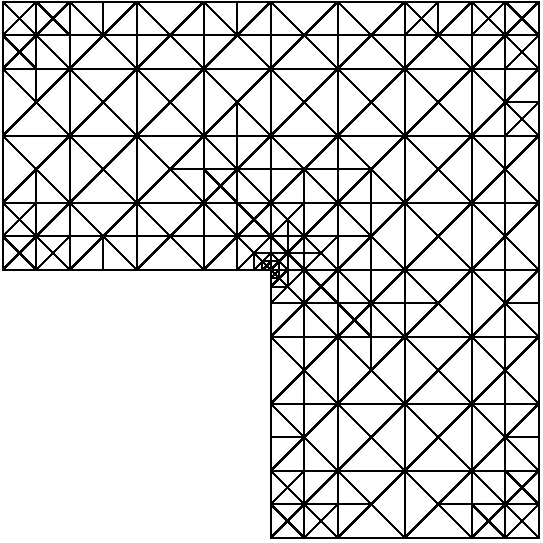
\includegraphics[width=.49\linewidth]{lshape_afem.png}
  \includegraphics[width=.49\linewidth]{crackone_afem.png}
  \caption{The left image corresponds to the L-shaped domain, the right corresponds to the cracked domain. Three methods are
  compared by plotting the approximation error $\uaenorm{\tilde U_k - U_K}_\O$ against the number of vertices. The adaptive methods
  used D\"orfler marking $\theta = 1/2$.}
  \label{fig:afem}
\end{figure}

\subsection{Mixed finite element solution}
Prager and Synge' theorem provided us with the following upper bound:
\[
  \enorm{u - U_h}_{\O}^2  \leq \norm{\nabla U_h - \vsig}^2_{\O} \quad \text{ for } \vsig \in H(\div; \O) \text{ s.t. } \div \v{\sigma} + f = 0
\]
The equilibrated method constructs $\v{\zeta} \in \RT_p(\O)$ such that $-\v{\zeta}$ satisfies the equilibrium condition, and thus we find an
upper bound in terms of $\nabla U_h + \v{\zeta}$. As noted before, the best upper bound with $\vsig \in \RT_p(\O)$ is found by minimizing
$\norm{\nabla U_h - \vsig}^2_{\O}$ for all fluxes $\vsig$ that are in equilibrium. Since this method is too expensive for an estimator
calculation the alternative of solving local minimization problems was introduced. The mixed finite element method provides the $\vsig$ that 
globally minimizes this norm. It is therefore interesting to compare their performance.



\end{document}
